%% LaTeX-Beamer template for KIT design
%% by Erik Burger, Christian Hammer
%% title picture by Klaus Krogmann
%%
%% version 2.1
%%
%% mostly compatible to KIT corporate design v2.0
%% http://intranet.kit.edu/gestaltungsrichtlinien.php
%%
%% Problems, bugs and comments to
%% burger@kit.edu

\documentclass[18pt]{beamer}
\def\tempfolder{../template/}
%% SLIDE FORMAT

% use 'beamerthemekit' for standard 4:3 ratio
% for widescreen slides (16:9), use 'beamerthemekitwide'
\usepackage{\tempfolder beamerthemekit}
% \usepackage{templates/beamerthemekitwide}

% -- Settings --------------------------------------------------------%
\setbeamertemplate{navigation symbols}{}

\def\figfolder{../figs/}
\def\logofolder{\tempfolder logo/}

\newcommand{\playIcon}{%
	
\begin{tikzpicture}[scale=0.5]
	\fill[fill=black] (0,0) -- (1.5,1) -- (0, 2) -- (0, 0);
	\end{tikzpicture}}


\usepackage{animate}
\usepackage{pdflscape}
\usepackage{pdfpages}
\usepackage{framed, color}
\usepackage{color}
\usepackage{tikz}
\usepackage{graphicx}
%\usepackage{subcaption}
\usepackage{listings}
\usepackage{tabulary}
\usepackage{tabularx}
\usepackage{qrcode}
\usepackage[utf8]{inputenc}

\usepackage{animate}
\usepackage{color}

\usetikzlibrary{shapes}
\usetikzlibrary{calc}

%% TITLE PICTURE
%\titleimage{mypicture}

%% TITLE LOGO
%\titlelogo{mylogo}

%% TikZ INTEGRATION
% use these packages for PCM symbols and UML classes
% \usepackage{templates/tikzkit}
% \usepackage{templates/tikzuml}

% the presentation starts here

\title[Group 3]{4D visualisation of the tropopause, identification of air mass exchanges and their fate}
\subtitle{Department of Mathematics \& Steinbuch Centre for Computing}
\author{Tianbai Xiao}

\institute{MathSEE Modeling Week}

%---------------------------------------------------------------------------------
\begin{document}
	
	\selectlanguage{english}
	
	%title page
	\titleimage{\tempfolder logo/background}
	\titlelogo{\tempfolder logo/MathSEE}
	%----------------------------------------------------------%
	
	%----------------------------------------------------------%
	% titlepage
	\maketitle

	%----------------------------------------------------------%
	%----------------------------------------------------------%
	
	
	\begin{frame}
	
	\frametitle{Self intro}
	\textbf{Tianbai Xiao}
	\begin{itemize}
		\item Postdoc in Department of Mathematics and Steinbuch Centre for Computing
		\item Ph.D. from Peking University and Research Assistant of Hong Kong University of Science and Technology
		\item  1) numerical and applied analysis, kinetic theory of gases, uncertainty quantification; 2) multiscale modeling and computational study of fluid mechanics, photon transports and plasma physics
	\end{itemize}
	
	\begin{figure}
		\begin{minipage}{0.45\linewidth}
			\centering
			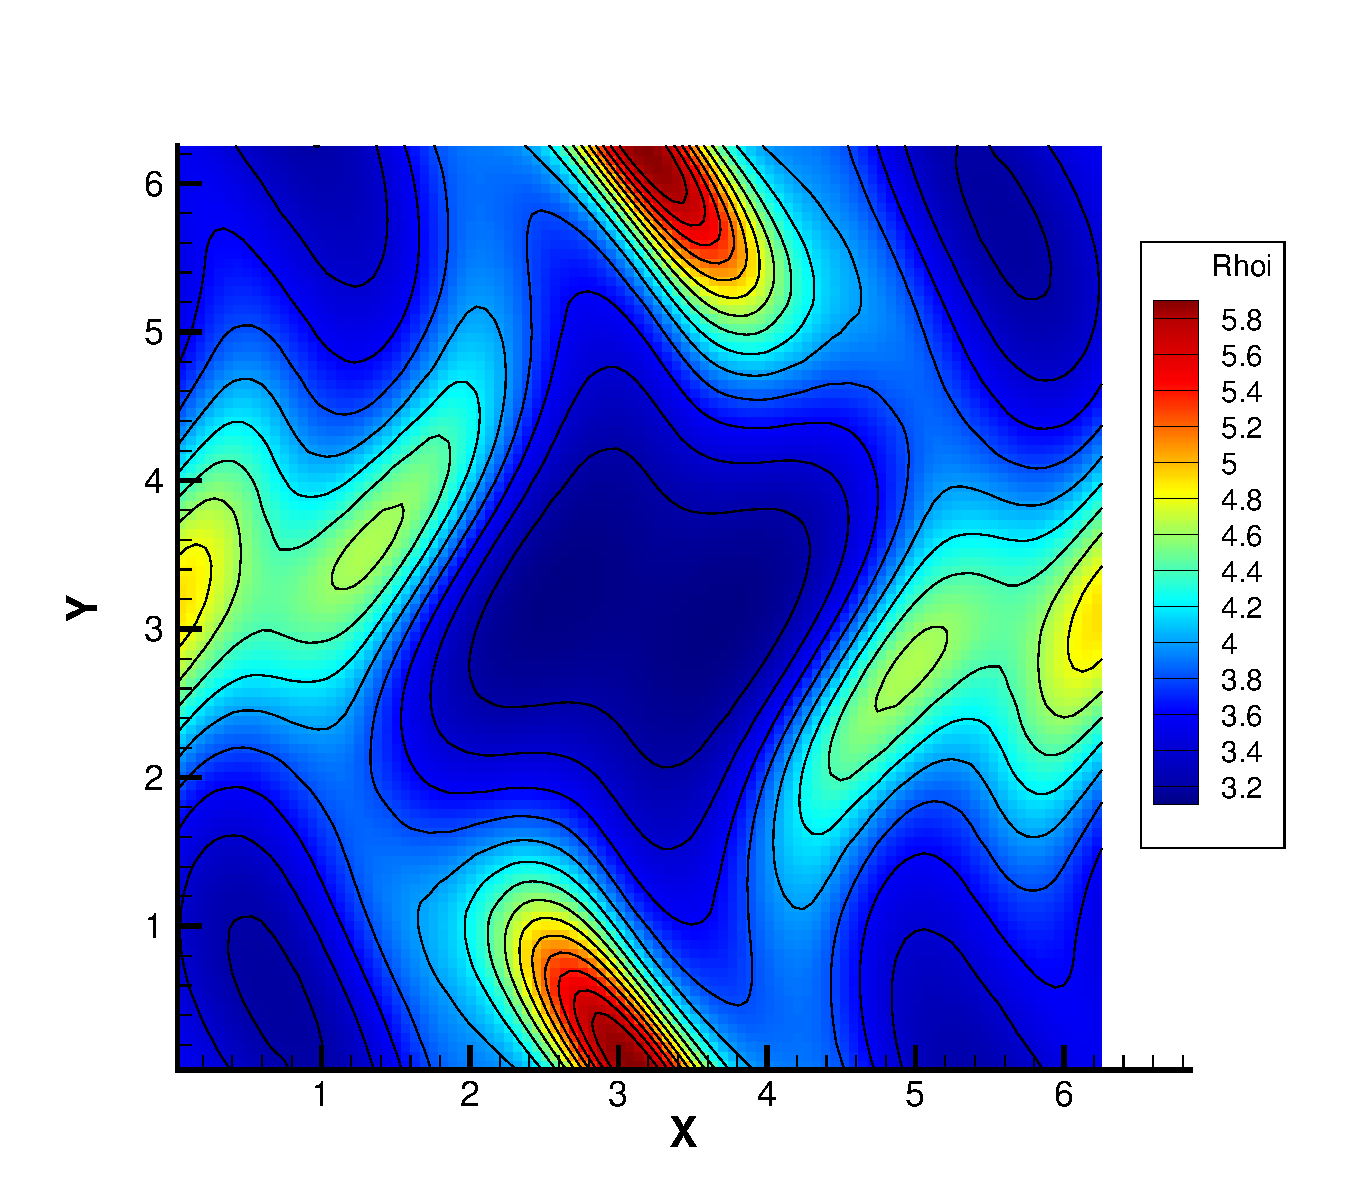
\includegraphics[width=0.8\textwidth]{orszag-tang.pdf}
		\end{minipage}
		\hfill
		\begin{minipage}{0.45\linewidth}
			\centering
			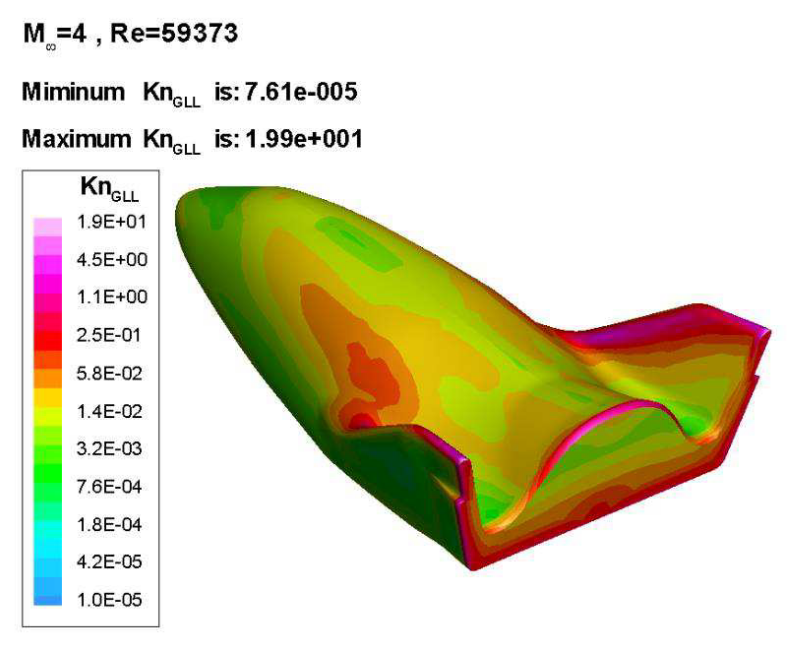
\includegraphics[width=0.8\textwidth]{kn-shuttle.png}
		\end{minipage}
	\end{figure}

	\end{frame}


	\begin{frame}
	
		\frametitle{Project intro}

		Atmospheric structure: multi-layer and multi-physics dynamics (roland.ruhnke@kit.edu \& jennifer.schroeter@kit.edu)

		%\vspace{3mm}
		
		\begin{figure}
			\begin{minipage}{0.45\linewidth}
				\centering
				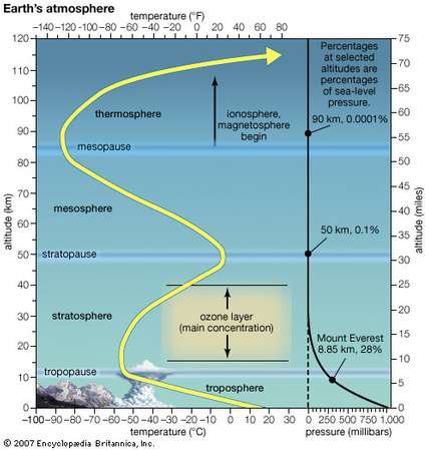
\includegraphics[width=0.8\textwidth]{../figs/atmospheric-layers.png}
			\end{minipage}
			\hfill
			\begin{minipage}{0.45\linewidth}
				\centering
				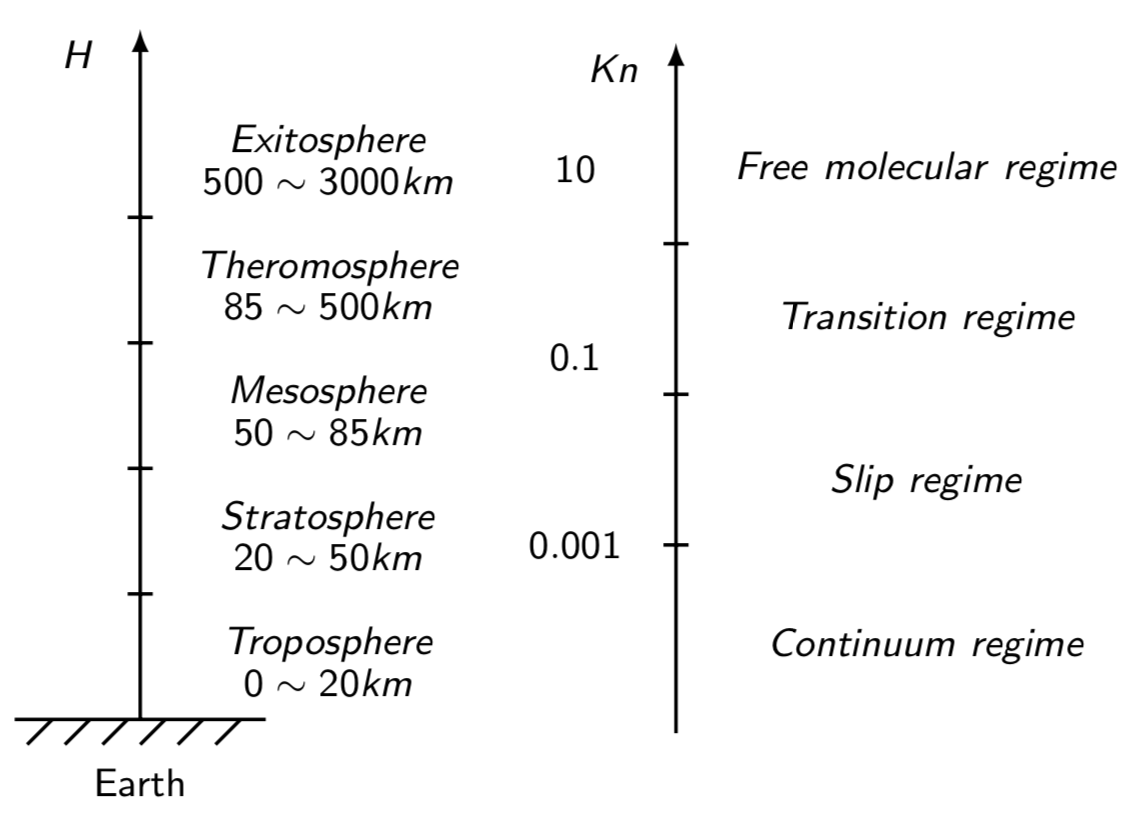
\includegraphics[width=1.0\textwidth]{atmosphere.png}
			\end{minipage}
		\end{figure}
		
		Tropopause: 
		\begin{itemize}
			\item key region for radiative forcing of greenhouse gases
			\item highly dynamical interface in space and time
		\end{itemize}
	
	\end{frame}


	\begin{frame}
	
		\frametitle{Research facility}
		The processes at the polar tropopause region have been investigated in a couple of research flights with the German HALO aircraft with the POLSTRACC campaign (see http://www.halo.dlr.de/science/missions/polstracc/polstracc.html)
		
		\begin{itemize}
			\item \small{GLORIA: Gimballed Limb Observer for Radiance Imaging of the Atmosphere}
			\item \small{ICON-ART: Numerical Simulator}
		\end{itemize}
	
		\begin{figure}
			\centering
			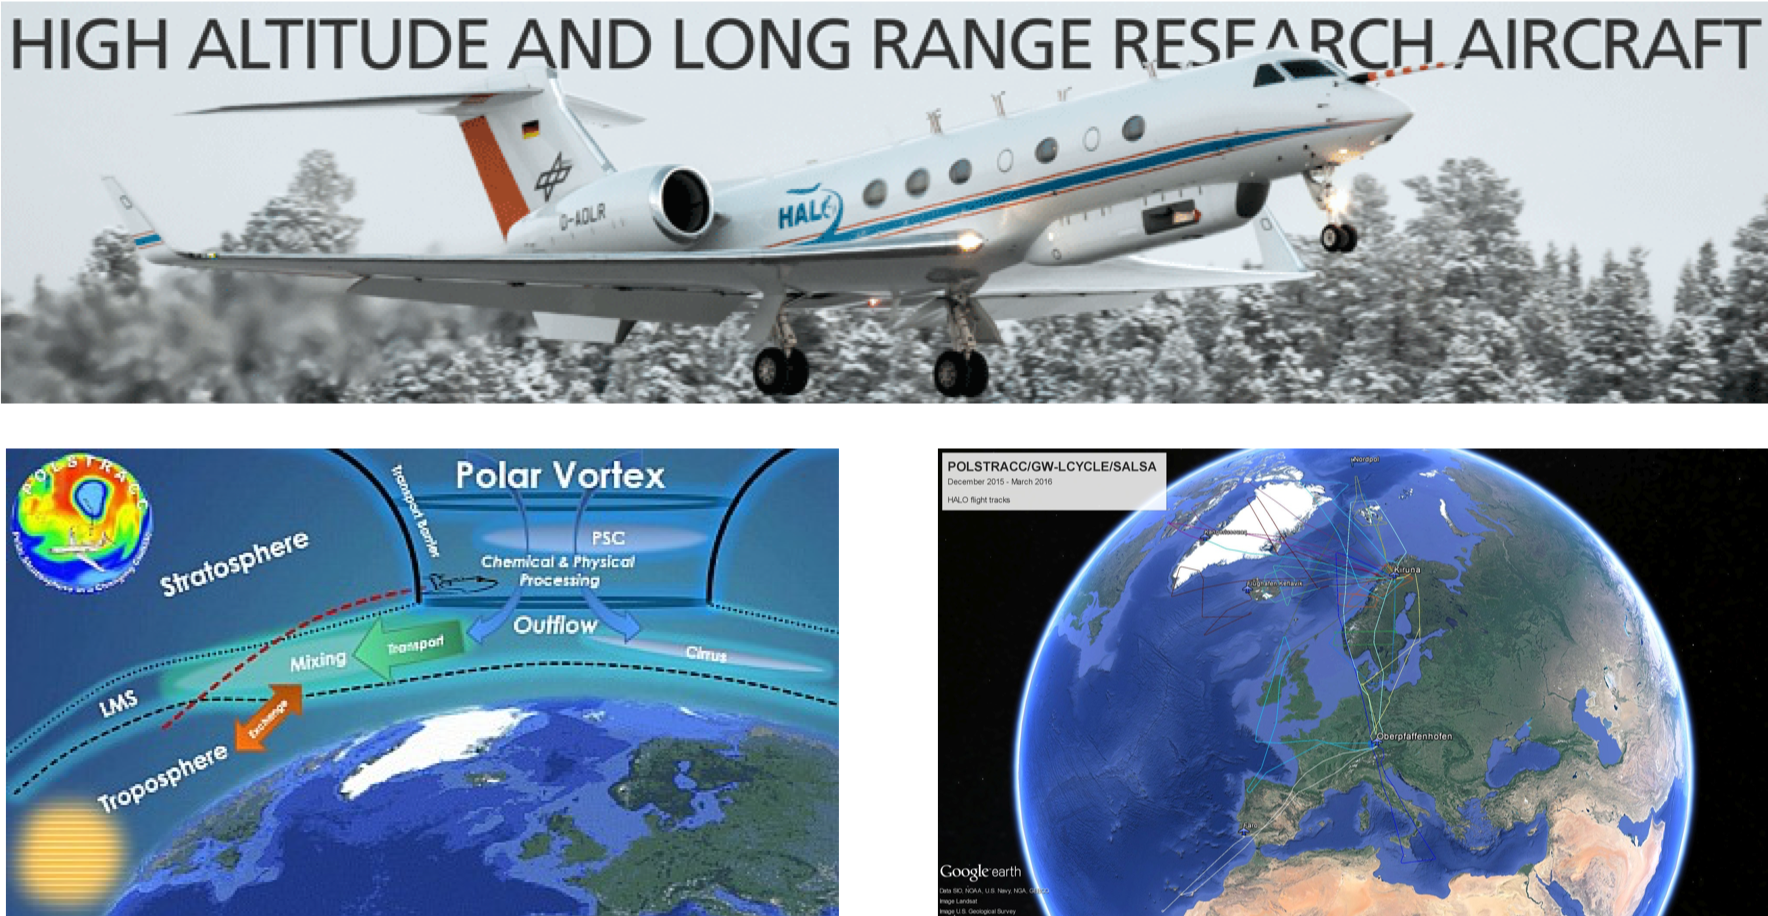
\includegraphics[width=0.5\textwidth]{airplane.png}
			
		\end{figure}
		
	\end{frame}

	
	\begin{frame}
	\frametitle{Results: wind speed, altitude and qv near 10 km}
	% ----------------分栏的结构开始---------------- %
	% 该结构中使用block分开两个内容区
	
	\begin{columns}
		\column{.5\textwidth}
		\begin{block}{}
			\begin{figure}
				\centering
				% Requires \usepackage{graphicx}
				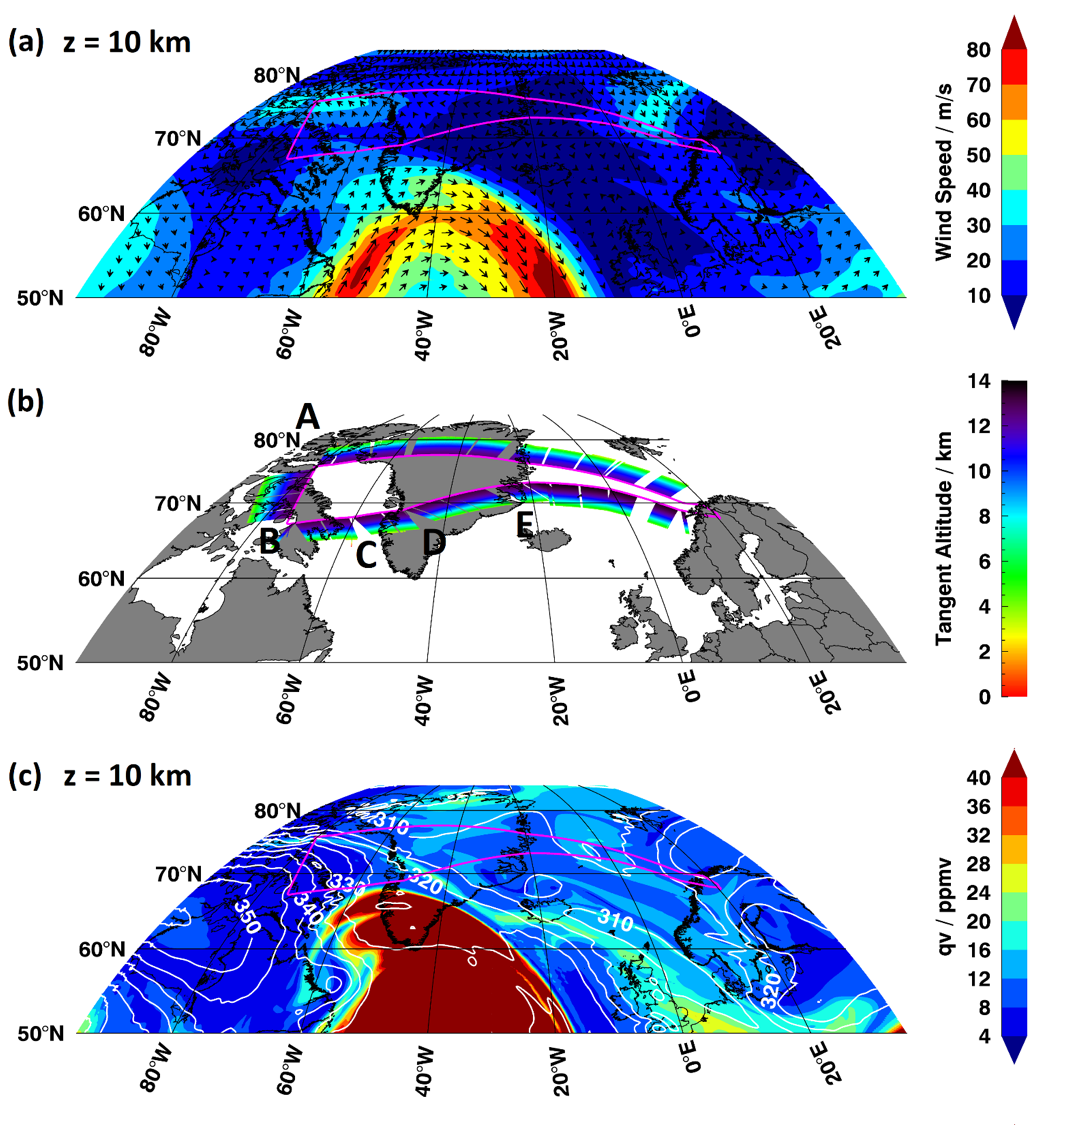
\includegraphics[width=0.8\textwidth]{polarpic1.png}
				\caption{\scriptsize {Meteorological situation and GLORIA sampling during HALO flight N.14 on Feb. 26, 2016. HALO flight track indicated by magenta line in all panels.}
				}
			\end{figure}
		\end{block}
		\column{.5\textwidth}
		\begin{block}{}
			\begin{itemize}
				\item \small{(a) ICON-ART simulated horizontal wind speed (colour-coded contour and arrows) at 10 km altitude }
				\item \small{(b) GLORIA measurement tangent points, colour-coded with altitude}
				\item \small{(c) ICON-ART simulated specific humidity qv (colour-coded contour) and potential temperature (white contour lines) at 10 km altitude}
			\end{itemize}
		The area within the strong horizontal wind gradient is associated with high values of specific humidity indicating tropospheric air at 10 km altitude.  
		\end{block}
	\end{columns}
	% ----------------分栏的结构结束---------------- %
	
	\end{frame}


	\begin{frame}
	\frametitle{Results: Potential Vorticity at different altitudes}
	% ----------------分栏的结构开始---------------- %
	% 该结构中使用block分开两个内容区
	
	\begin{columns}
		\column{.5\textwidth}
		\begin{block}{}
			\begin{figure}
				\centering
				% Requires \usepackage{graphicx}
				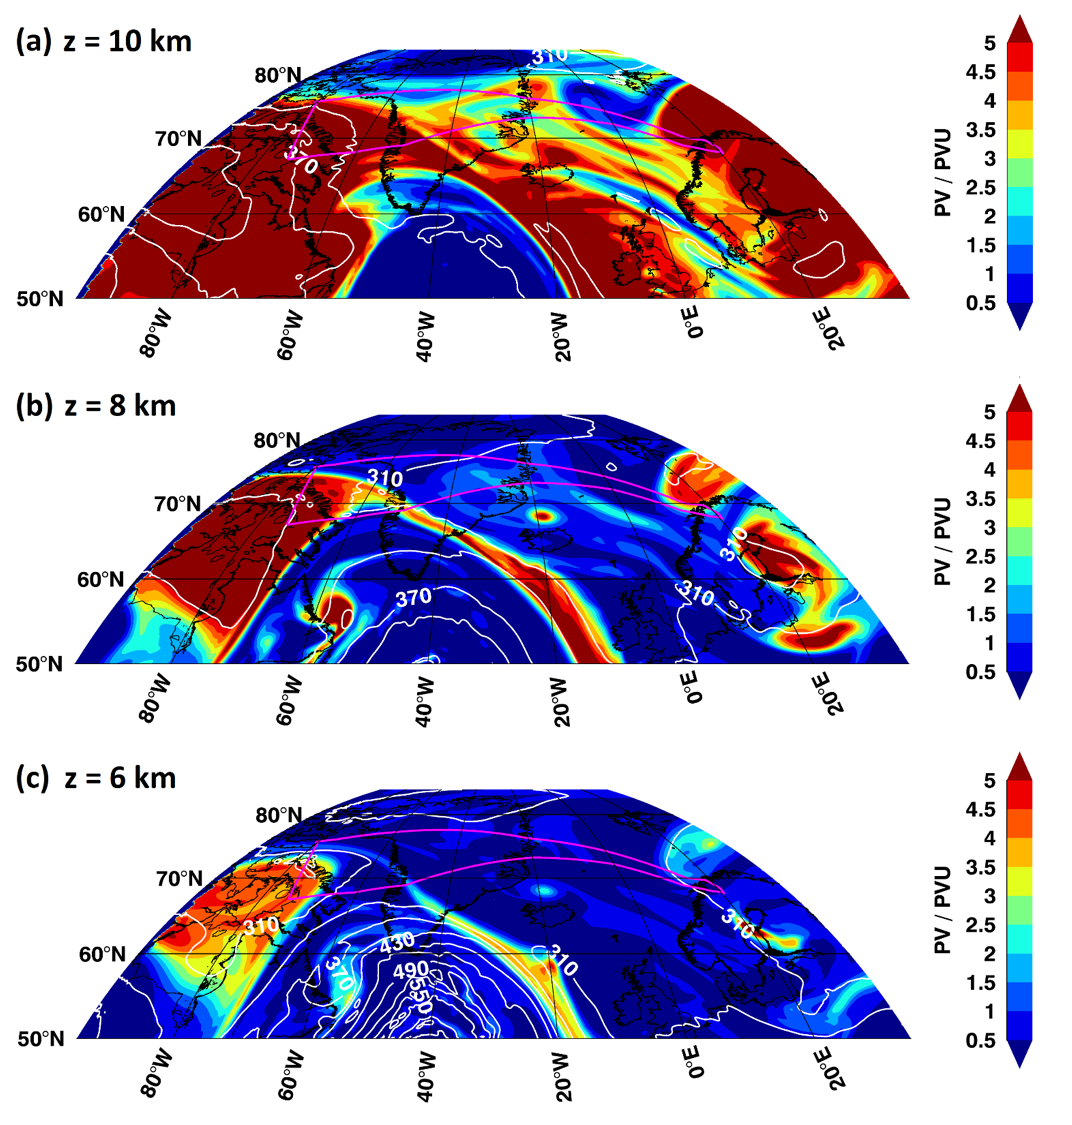
\includegraphics[width=0.7\textwidth]{polarpic2.png}
				\caption{\scriptsize {ICON-ART potential vorticity (colour-coded contour) and equivalent potential temperature (white contour lines) at different altitudes. HALO flight track indicated by magenta line in all panels. }
				}
			\end{figure}
		\end{block}
		\column{.5\textwidth}
		\begin{block}{}
			\begin{itemize}
				\item A PVU value of 2 can act as a measure for the tropopause.
				\item The high values of specific humidity corresponds to low values of PV at 10 km altitude. 
				\item Below 10 km high values of PV are visible indicating stratospheric air at these altitudes.
			\end{itemize}
		\end{block}
	\end{columns}
	% ----------------分栏的结构结束---------------- %
\end{frame}


	\begin{frame}
	\frametitle{Results: vertical cross-section of PV}
	% ----------------分栏的结构开始---------------- %
	% 该结构中使用block分开两个内容区
	
		\begin{columns}
			\column{.5\textwidth}
			\begin{block}{}
				\begin{figure}
					\centering
					% Requires \usepackage{graphicx}
					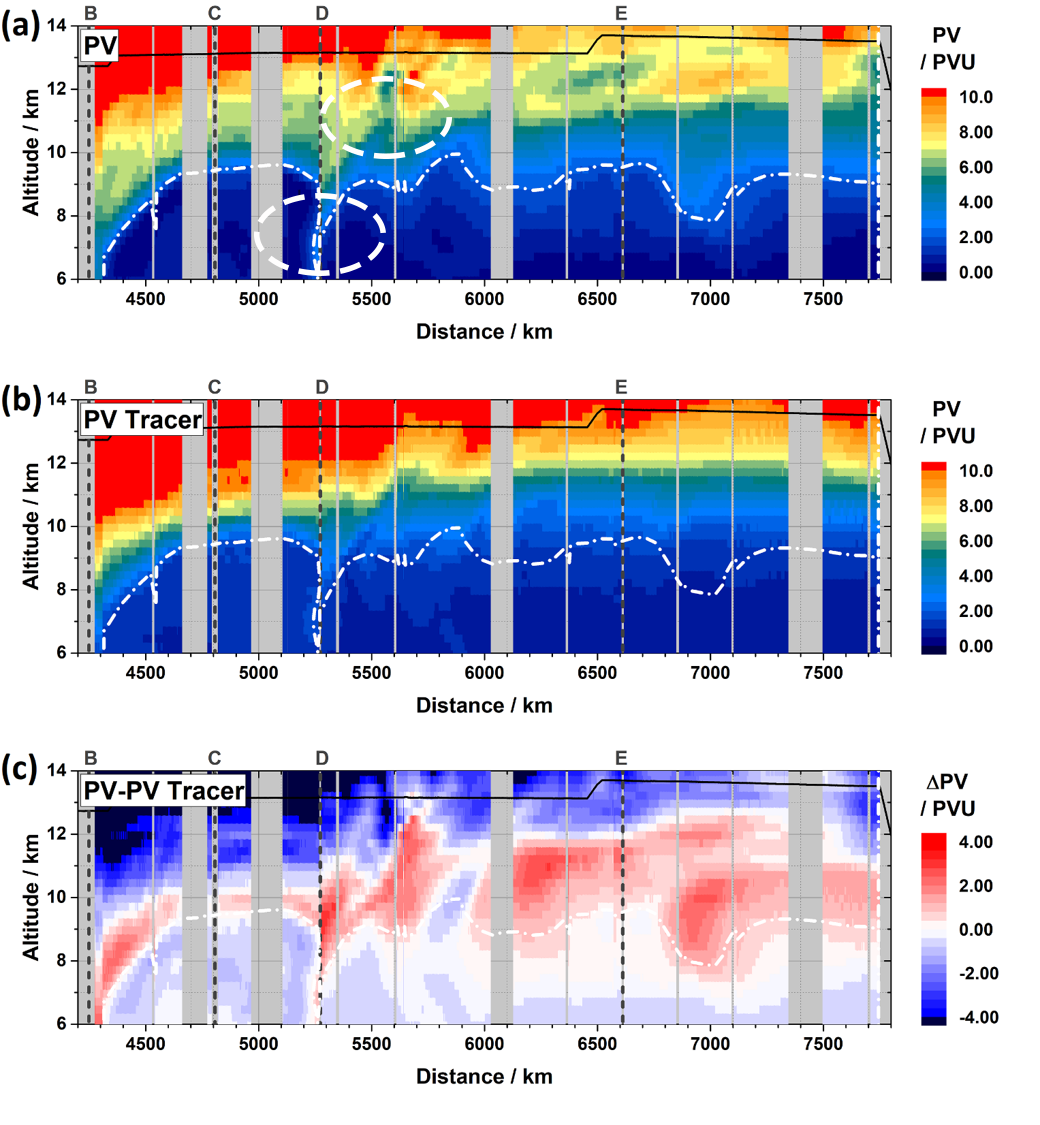
\includegraphics[width=5cm]{../figs/cross-section.png}
					\caption{\footnotesize {Vertical cross-sections of (a) potential vorticity PV, (b) PV tracer, and (c) PV - PV tracer. }
					}
				\end{figure}
			\end{block}
			\column{.5\textwidth}
			\begin{block}{}
				\begin{itemize}
					\item \small{Dash-dotted white lines indicate the PV = 2 PVU level as indicator for the dynamical tropopause}
					\item \small{HALO flight altitude indicated by black line in all panels}
					\item \small{The two white circles shows features of interest along the flight track. A fast and sharp decrease in altitude of the tropopause accompanied by an uplift in short distance}
				\end{itemize}
			\end{block}
		\end{columns}
	% ----------------分栏的结构结束---------------- %
	\end{frame}


	\begin{frame}
	
		\frametitle{Results: air uplift and exchange}
		\large
		
		\begin{itemize}
			\item \small{This uplift of air masses with tropospheric characteristics above the dynamical tropopause is seen in measurements as well as in the model simulations}
			\item \small{ The question is \textcolor{red}{where does this exchange is generated} and \textcolor{red}{what is the fate of it}}
		\end{itemize}
		
		\begin{figure}
			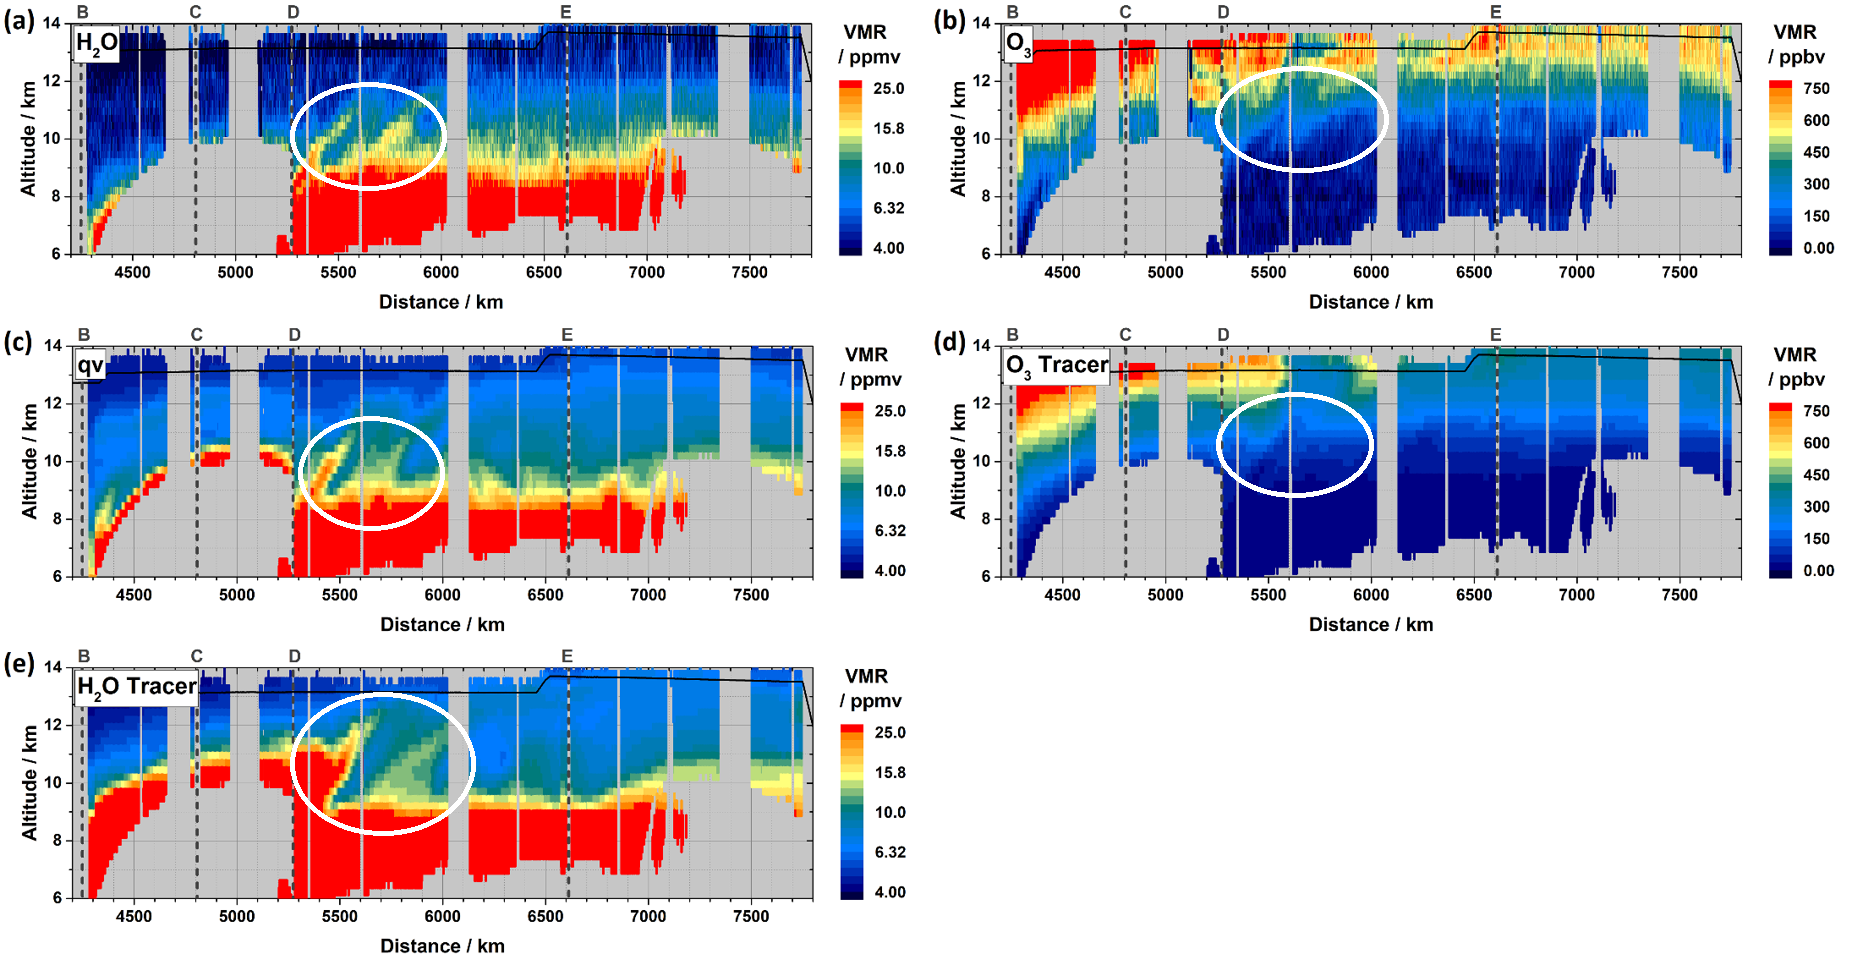
\includegraphics[width=0.55\textwidth]{../figs/uplift.png}
			\caption{\footnotesize {Fine-structures in GLORIA measurements and ICON-ART simulations. Vertical cross-sections along east-bound flight section. GLORIA (a) water vapour and (b) ozone, and ICON-ART (c) specific humidity, (d) ozone tracer, and (e) water vapour tracer at 18 UTC. HALO flight altitude indicated by black line in all panels. }
			}
		\end{figure}
		
	\end{frame}

	
	\begin{frame}
		\frametitle{Conclusion and work plan}
		\large

		\begin{itemize}
			\item 4D visualisation of tropopause represented by the simulated PV
			\item Automatic identification of air masses of tropospheric origin above the tropopause, e.g. by analysing the qv and the PV fields (\textcolor{red}{Q: where is the origin of this exchange of tropospheric air through the tropopause into the stratosphere})
			\item Tracking of these air masses in time and space to visualise their atmospheric fate (\textcolor{red}{Q: is the exchange reversible or not?})
			\item English speaking group
			\item My utmost to help (but no REPLACEMENT)
		\end{itemize}

	\end{frame}

	
\end{document}
% ---------------------------------------------------------------------------------
